\section{OpenMP}

\begin{frame}{From CSR to MergedCSR}
\begin{itemize}
  \item<1-> Graphs are usually stored in the Compressed Sparse Row format (CSR)
  % each access to neighbors' adjacency list requires two memory accesses
  \item<2-> MergedCSR core idea: access only \texttt{row\_ptr} array during BFS traversal
  \begin{itemize}
    \item<2-> \texttt{row\_ptr} array contains also algorithm-specific metadata (ex. distance)
  \end{itemize}
\end{itemize}
\only<1>{
\begin{figure}
  \centering
  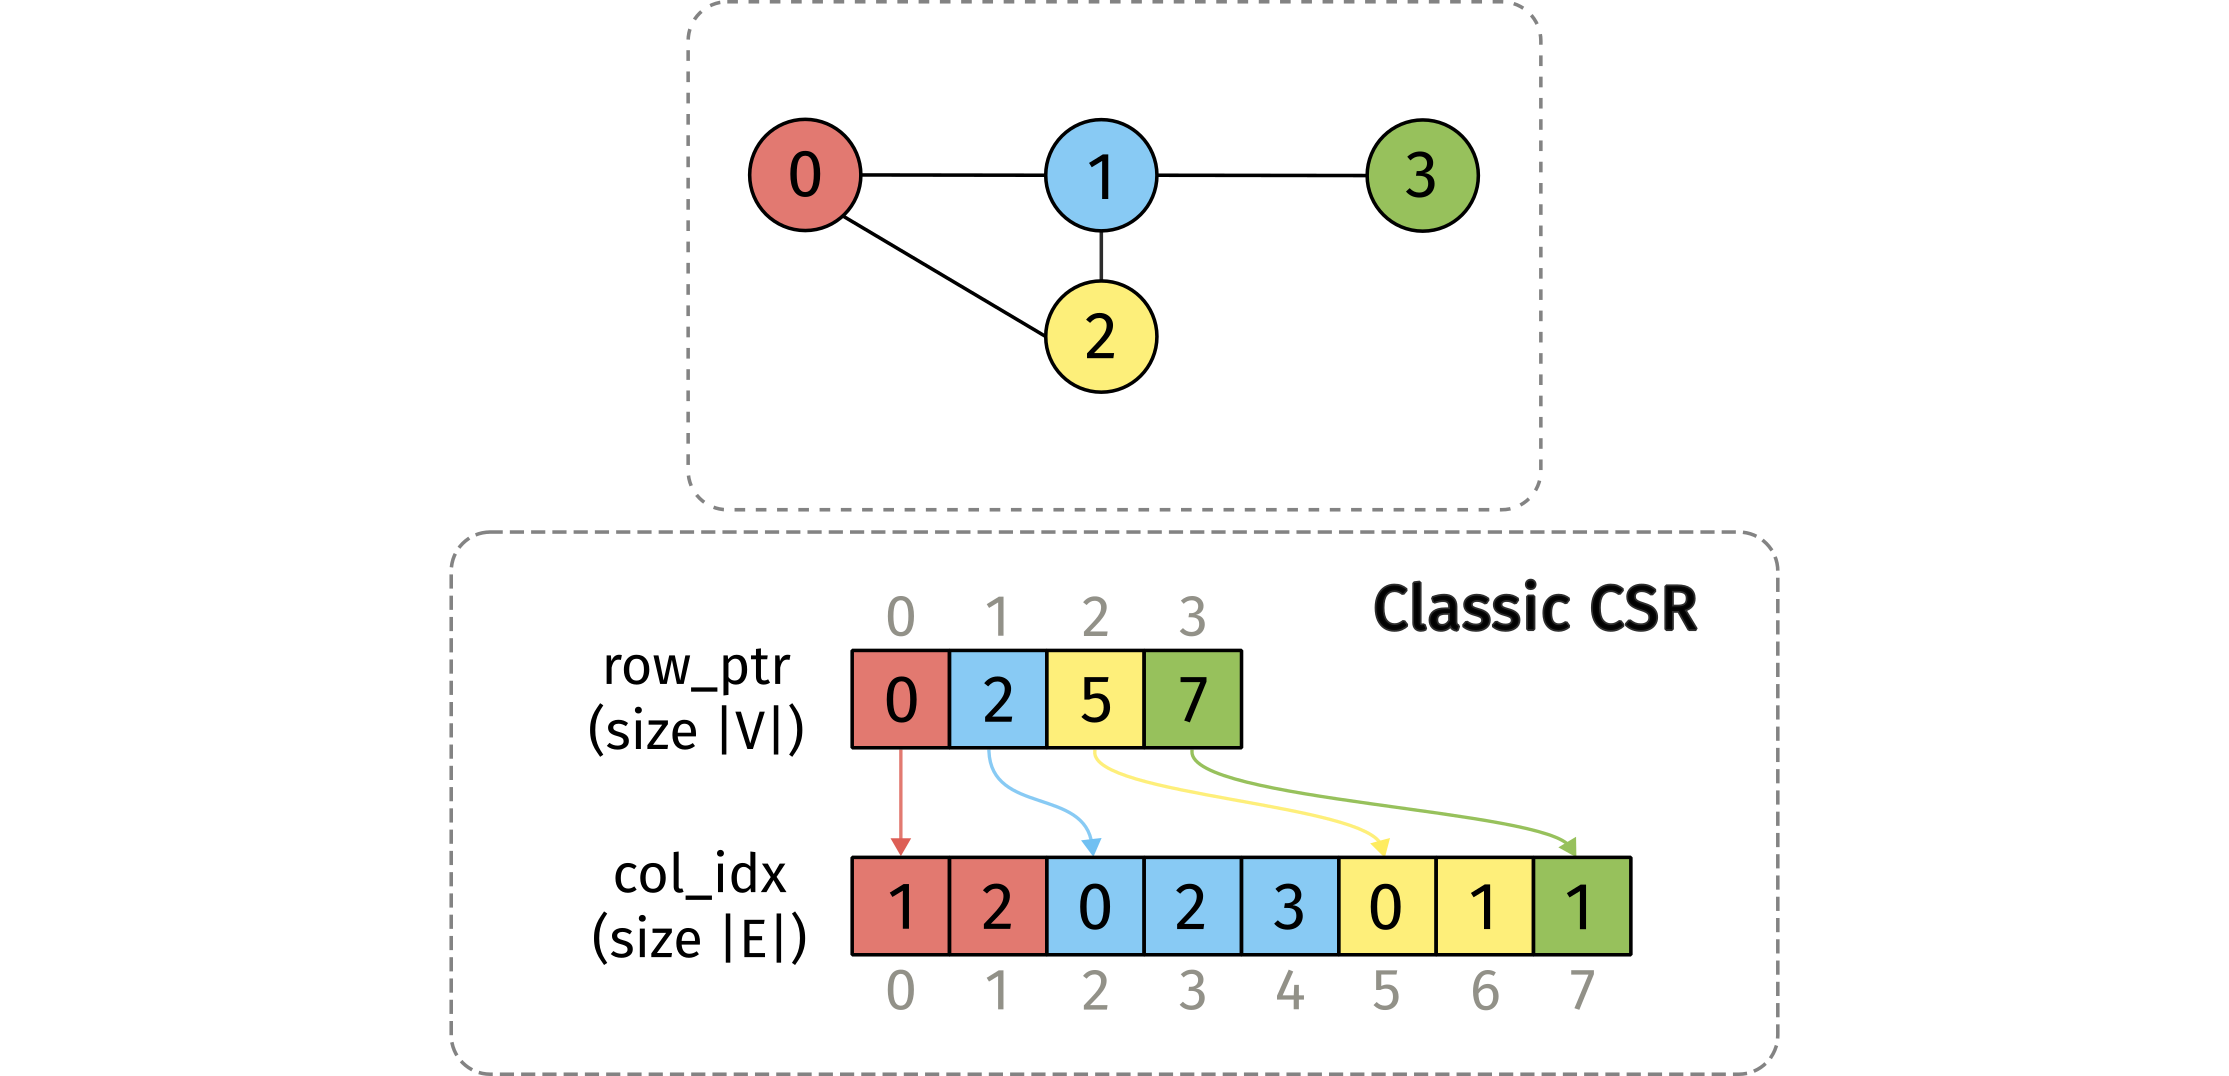
\includegraphics[width=0.8\linewidth]{images/csr_slides_1.png}
\end{figure}
}
\only<2>{
\begin{figure}
  \centering
  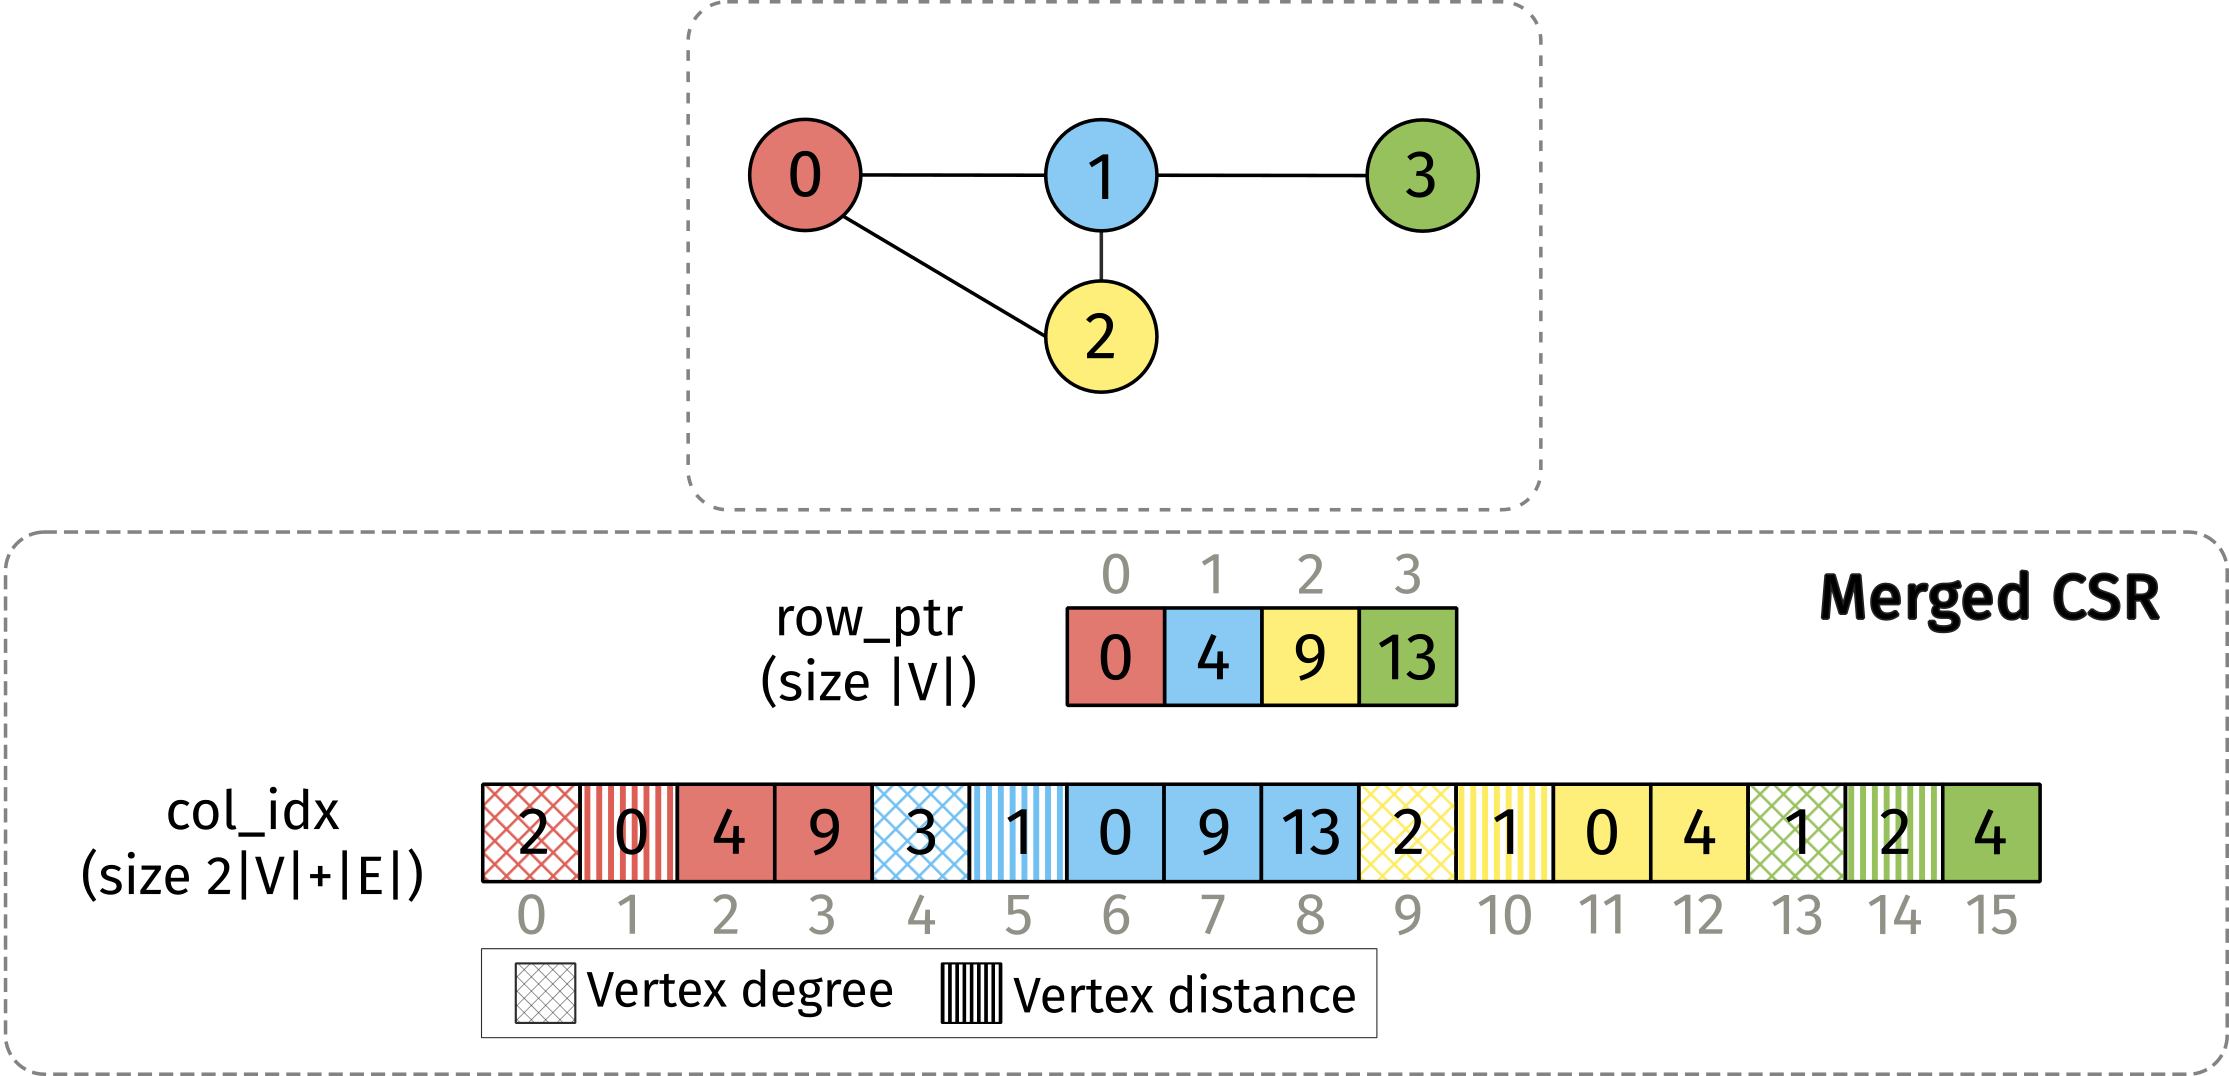
\includegraphics[width=0.8\linewidth]{images/csr_slides_2.png}
\end{figure}
}
\only<3>{
\begin{figure}
  \centering
  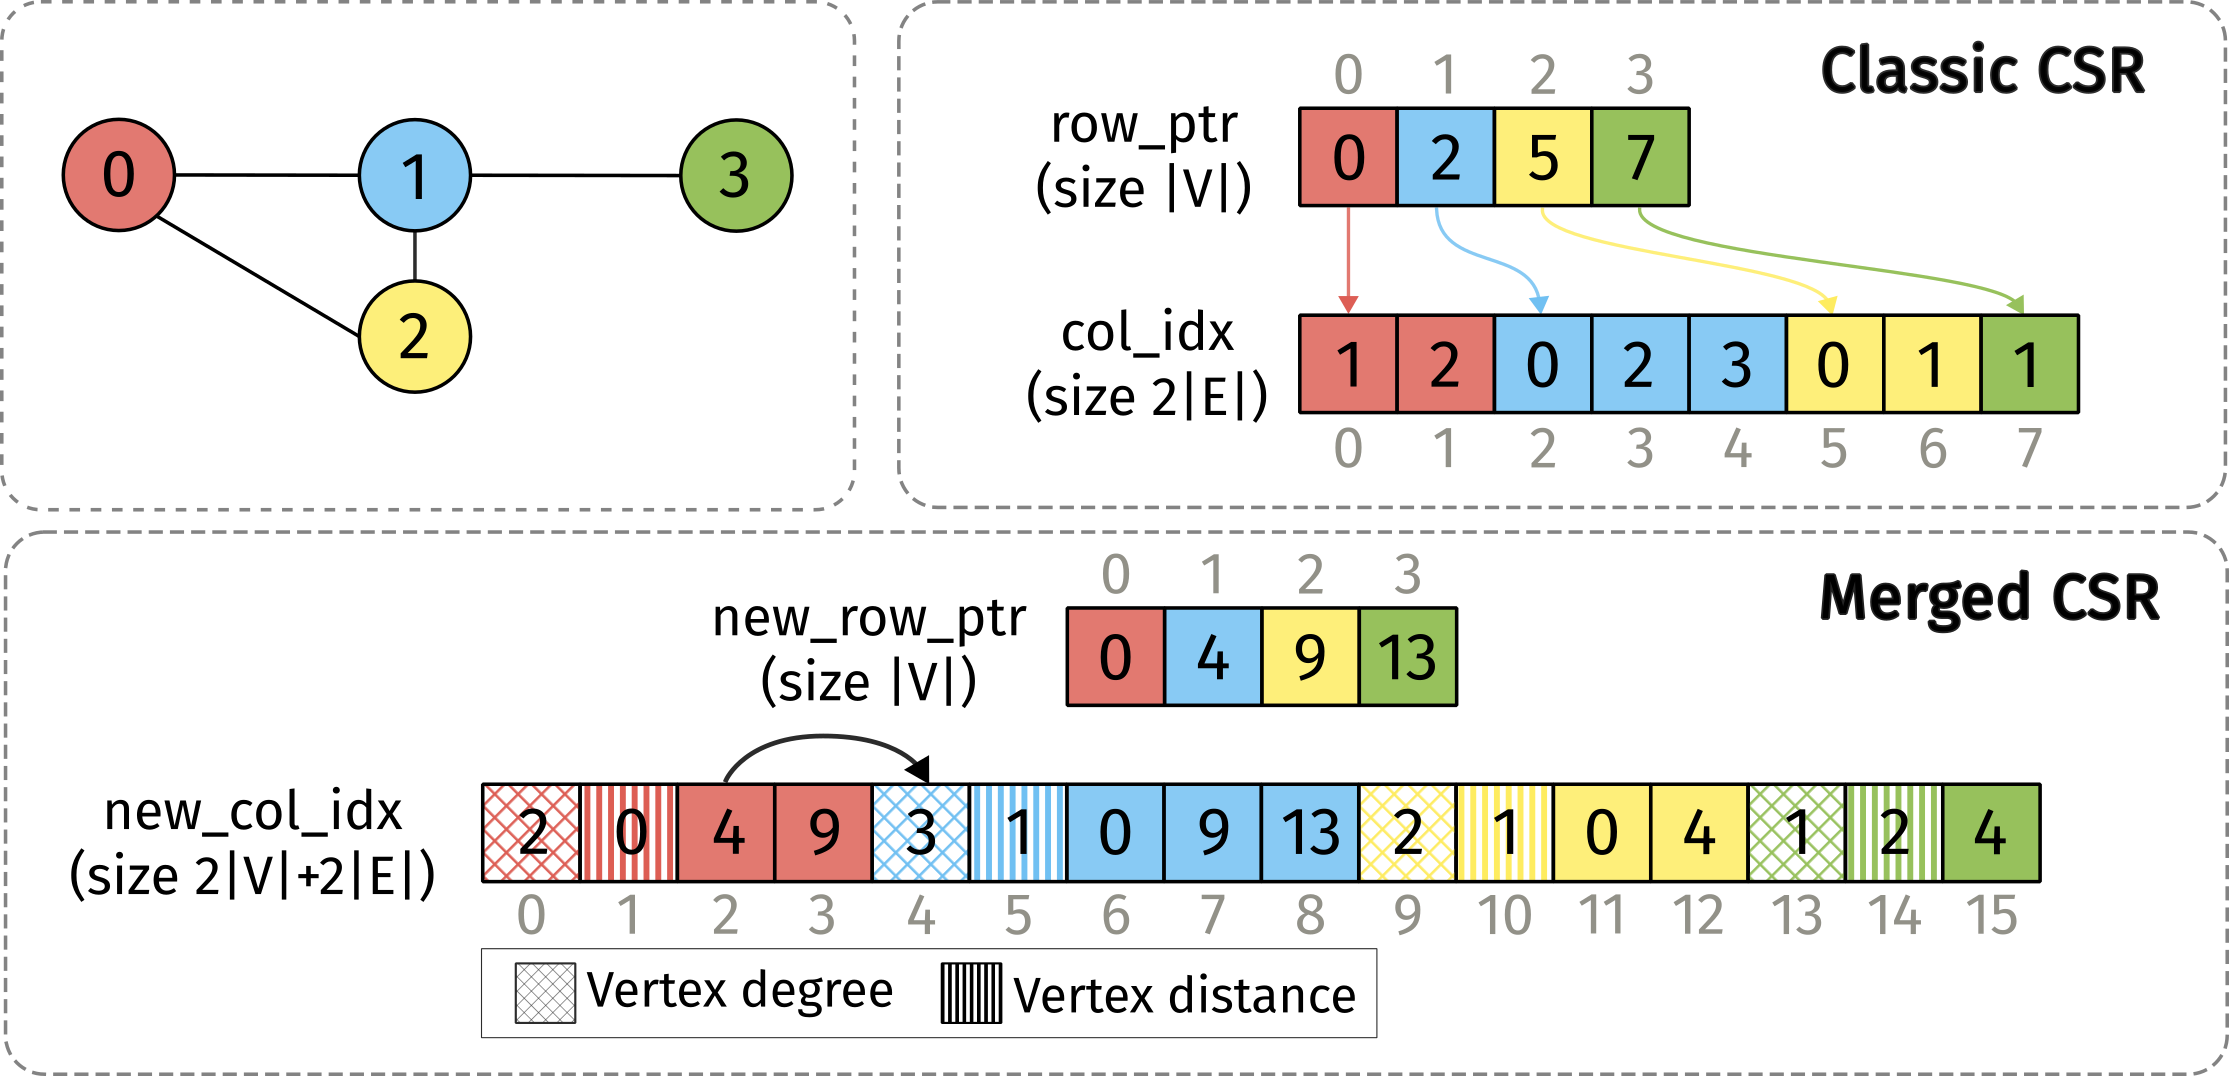
\includegraphics[width=0.8\linewidth]{images/csr_slides_3.png}
\end{figure}
}
\only<4>{
\begin{figure}
  \centering
  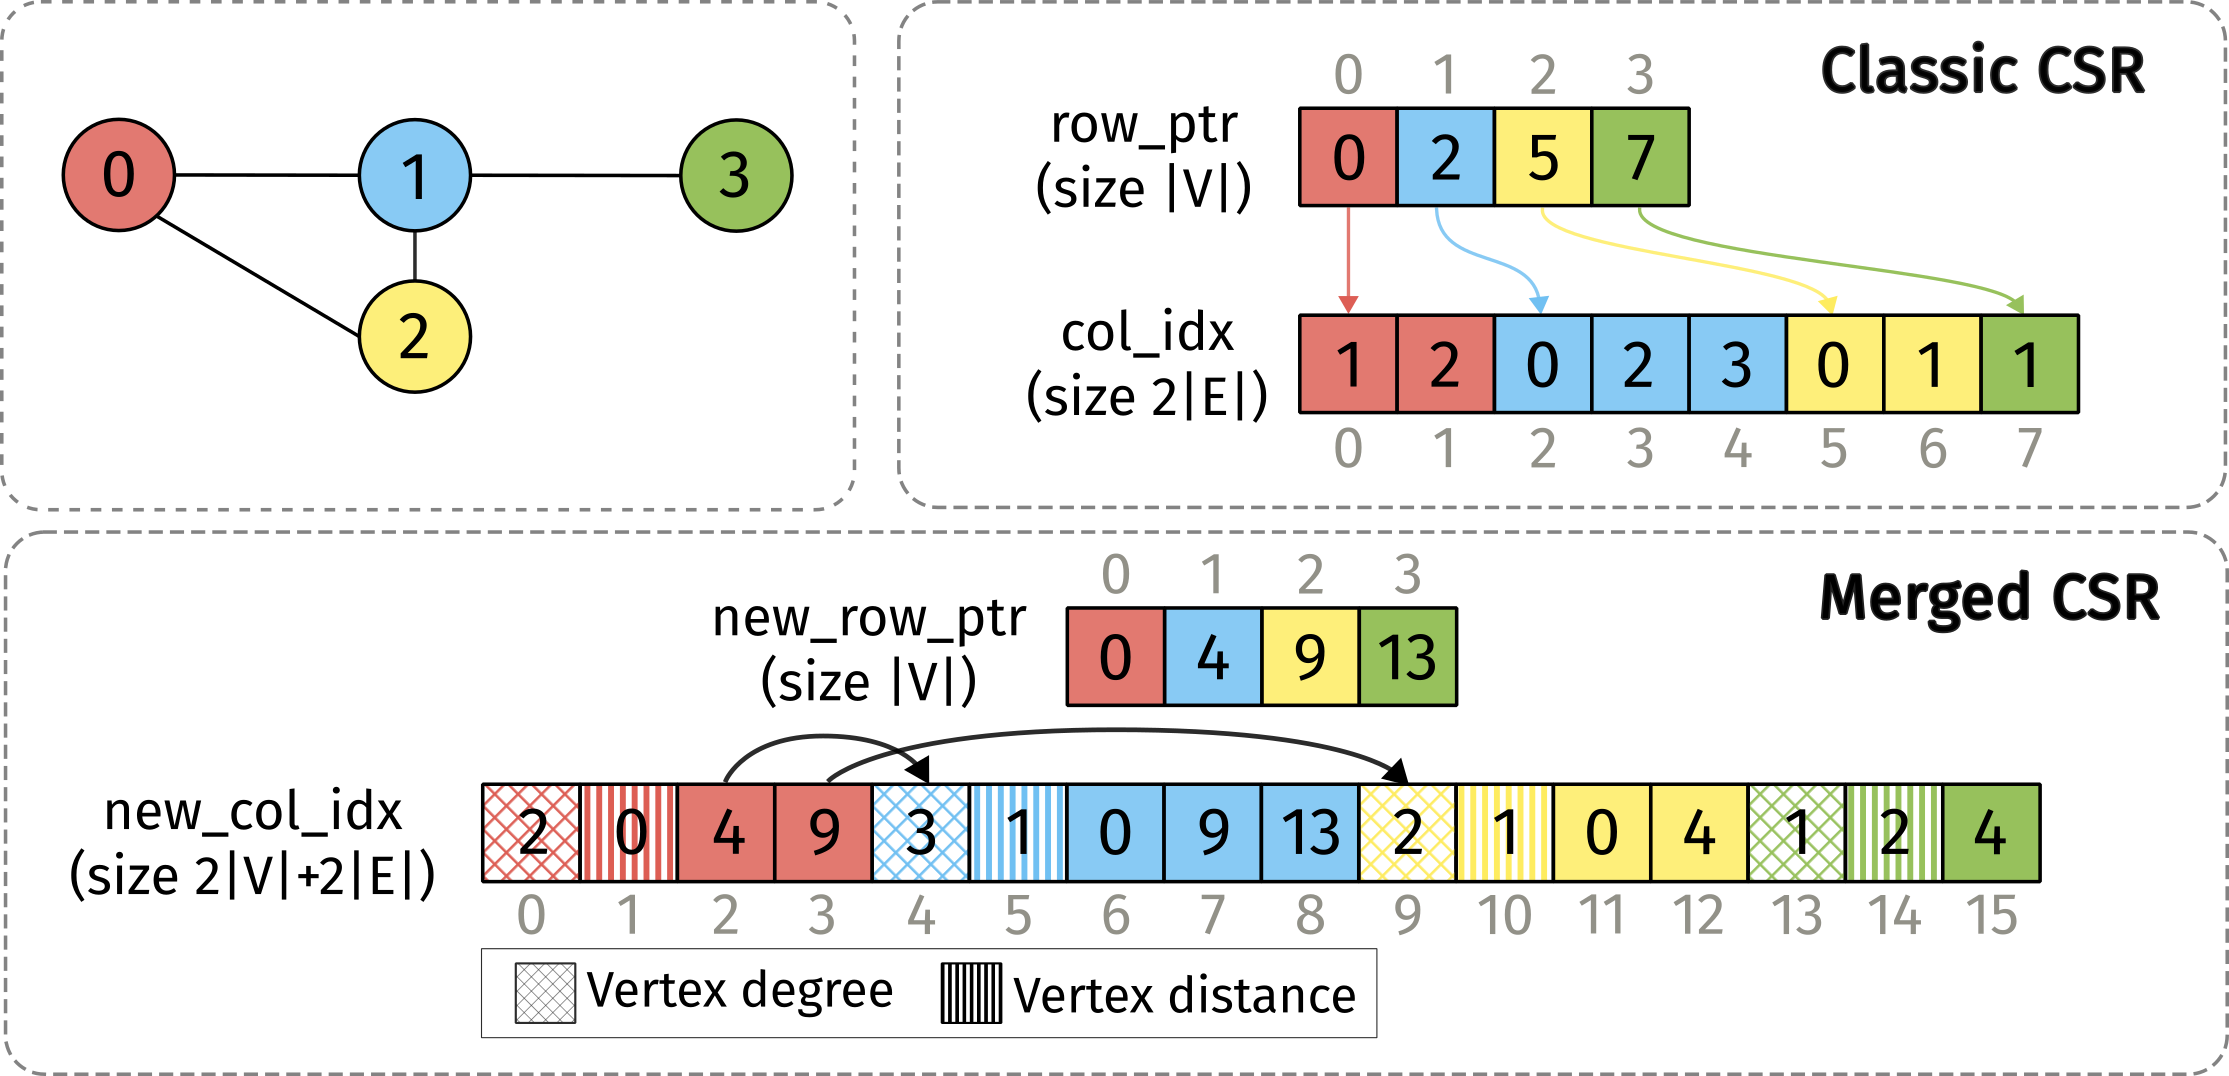
\includegraphics[width=0.8\linewidth]{images/csr_slides_4.png}
\end{figure}
}
\end{frame}

\begin{frame}[fragile]{OpenMP implementation}
  \begin{columns}[c]
  \begin{column}{0.5\textwidth}
  \begin{itemize}
    \item \textbf{OpenMP} is a widely used framework for \textbf{parallel programming} in C and C++
    \item Uses simple compiler directives called pragmas
  \end{itemize}
  \end{column}
  \begin{column}{0.5\textwidth}
  \centering
  \begin{minipage}[t]{\textwidth}
  \vspace{3mm}
  \begin{minted}[fontsize=\scriptsize, bgcolor=lightgray!30, breaklines]{c}
  #pragma omp parallel for reduction(vec_add : next_frontier)
  for (const auto &v : this_frontier) {
    // Process vertex v
  }
  \end{minted}
  \vspace{1.5mm}
  \end{minipage}
  \scalebox{0.9}{
  \begin{tikzpicture}[
    node distance=0.5cm,
    block/.style={
      rounded corners,
      draw,
      thick,
      align=center,
      font=\sffamily\bfseries\scriptsize,
      minimum width=1cm,
      minimum height=0.5cm
    },
    iteration_block/.style={
      rectangle,
      draw,
      thick,
      align=center,
      font=\sffamily\scriptsize,
      inner sep=5pt,
      text width=0.7cm,
      minimum height=1.2cm
    },
    gray_block/.style={
      block,
      fill=lightgray!50
    },
    arrow/.style={
      -Stealth,
      thick
    }
  ]
  
  % Nodes
  \node[block] (parallel_start) {start};
  
  \node[block, below=3mm of parallel_start] (for_start) {\#pragma omp parallel for};
  
  \node[iteration_block, below left=0.3cm and 0mm of for_start.south west] (iter1) {$v_1$\\$v_2$\\$v_3$};
  \node[iteration_block, below=0.3cm of for_start] (iter2) {$v_4$\\$v_5$\\$v_6$};
  \node[iteration_block, below right=0.3cm and 0mm of for_start.south east] (iter3) {$v_7$\\$v_8$\\$v_9$};
  
  \node[block, below=0.3cm of $(iter1.south)!0.5!(iter3.south)$] (for_end) {/* end omp for */};
  
  % Barrier line and text
  \coordinate (barrier_left) at ($(for_end.south west) - (0.2, 0.2)$);
  \coordinate (barrier_right) at ($(for_end.south east) + (0.2, -0.2)$);
  \draw[red, thick] (barrier_left) -- (barrier_right);
  \node[right=0.5mm of barrier_right, anchor=west, font=\scriptsize, red, align=center] {implicit\\barrier};
  
  \node[gray_block, below=0.5cm of for_end] (parallel_end) {Reduction\\\textit{(Merge frontiers)}};
  
  % Arrows
  \draw[arrow] (parallel_start) -- (for_start);
  
  % Arrows from for_start to iteration blocks
  \draw[arrow] (for_start) -| ($(iter1.north) + (0,0.5)$) -- (iter1);
  \draw[arrow] (for_start) -- (iter2);
  \draw[arrow] (for_start) -| ($(iter3.north) + (0,0.5)$) -- (iter3);
  
  % Arrows from iteration blocks to for_end
  \draw[arrow] (iter1.south) |- (for_end.west);
  \draw[arrow] (iter2.south) -- (for_end);
  \draw[arrow] (iter3.south) |- (for_end.east);
  
  \draw[arrow] (for_end) -- (parallel_end);
  
  \end{tikzpicture}
  }
  \end{column}
  \end{columns}
  \end{frame}

% \begin{frame}{Parallelization strategies}
% \begin{itemize}
%   \item Different parallelization strategies, depending on the graph type
%   \item Strategy used: Frontier partitioning + Merge step
% \end{itemize}
% \centering
% \vspace{0.3cm}
% \scalebox{0.9}{
% \begin{tikzpicture}[
%   % Global styles
%   node distance=1.5cm, % Vertical distance between layers
%   block_style/.style={
%     rounded corners=3pt, % Slightly rounded corners
%     draw, % Black border
%     thick, % Thicker border
%     align=center,
%     font=\sffamily\small,
%     minimum height=0.8cm,
%     inner xsep=5pt, % Horizontal padding
%     outer sep=0pt % No extra outer spacing
%   },
%   frontier_node/.style={
%     block_style,
%     fill=gray!10 % Light gray fill for frontier nodes
%   },
%   thread_node/.style={
%     block_style,
%     fill=orange!30 % Orange fill for thread nodes
%   },
%   merge_node/.style={
%     block_style,
%     fill=green!20 % Light green fill for merge node
%   },
%   arrow/.style={
%     -Stealth, % Arrow tip style
%     thick % Thicker arrows
%   }
% ]

% % Nodes
% \node[frontier_node, minimum width=4cm] (current_frontier) {Current Frontier};

% \node[thread_node, below left=0.5cm and 1.5cm of current_frontier.south] (thread1_left) {Thread 1};
% \node[thread_node, below=0.5cm of current_frontier.south] (thread2) {Thread 2};
% \node[thread_node, below right=0.5cm and 1.5cm of current_frontier.south] (thread1_right) {Thread 3};

% \node[merge_node, below=0.5cm of thread2.south, minimum width=3cm] (merge_step) {Merge Next Frontier}; % Adjust vertical position and width

% \node[frontier_node, below=0.3cm of merge_step, minimum width=4cm] (next_frontier) {Start new iteration with Next Frontier};

% % Arrows
% % From Current Frontier to Threads
% \draw[arrow] (current_frontier.west) -| (thread1_left.north);
% \draw[arrow] (current_frontier.south) -| (thread2.north);
% \draw[arrow] (current_frontier.east) -| (thread1_right.north);

% % From Threads to Merge Step
% \draw[arrow] (thread1_left.south) |- (merge_step.west);
% \draw[arrow] (thread2.south) -| (merge_step.north);
% \draw[arrow] (thread1_right.south) |- (merge_step.east);

% % From Merge Step to Next Frontier
% \draw[arrow] (merge_step.south) -- (next_frontier.north);

% \end{tikzpicture}
% }
% \end{frame}

% \begin{frame}[fragile]{Implementation}
% % schedule(static)
% \begin{minted}[fontsize=\small, bgcolor=lightgray!30, breaklines]{cpp}
% #pragma omp declare reduction(vec_add : \
%   omp_out.insert(omp_out.end(), omp_in.begin(), omp_in.end()))

% #pragma omp parallel for reduction(vec_add : next_frontier) if(this_frontier.size() > 50)
% for (const auto &v : this_frontier) {
%   // Process vertex v
% }
% \end{minted}
% \end{frame}

\begin{frame}{Inefficiencies of the OpenMP implementation}
  \begin{itemize}
    \item Merging step is not parallel
    \pause
    \item In graphs with large diameter, OpenMP enters the \texttt{parallel for} region more than 10k times for a single BFS runs
  \end{itemize}
\end{frame}